\section{Definições L-atribuídas}

\begin{frame}[fragile]{Ordem de avaliação dos atributos}

    \begin{itemize}
        \item Quando a tradução acontece durante a análise sintática, a ordem de avaliação dos atributos está ligada à ordem de construção dos nós da
            árvore gramatical
       %\pause

        \item Uma ordem natural, que ocorre frequentemente em muitos métodos de tradução \textit{top-down} e \textit{bottom-up}, é baseada em uma
            travessia em profundidade
       %\pause

        \item Nesta ordem, os atributos herdados dos filhos do nó são todos computados antes que os atributos sintetizados do nó sejam computados
       %\pause

        \item Mesmo que a árvore sintática não seja construída explicitamente, é importante compreender a ordem de avaliação dos atributos de seus nós
            e sua relação com travessias em profundidade
    \end{itemize}

\end{frame}

\begin{frame}[fragile]{Ordem natural de avaliaçao dos atributos}

    \begin{algorithmic}[i]
        \Require{Uma árvore sintática e o nó raiz, que deve ser o argumento da primeira chamada} 
        \Ensure{Os valores de todos os atributos dos nós}
        \vspace{0.2in}

        \Procedure{visit}{$node$}
            \For{cada filho $m$ de $node$, da esquerda para a direita}
                \State{avalie os atributos herdados de $m$}
                \State{\Call{visit}{$m$}}
            \EndFor
            \State{avalie os atributos sintetizados de $node$}
        \EndProcedure
    \end{algorithmic}

\end{frame}

\begin{frame}[fragile]{Definições L-atribuídas}

    \begin{block}{Definição}
        Uma definição dirigida pela sintaxe é L-atribuída (O L vem do inglês \textit{left}) se cada atributo herdado de $X_j, 1\leq j\leq n$, do lado direito da
        produção $A\to X_1X_2\ldots X_n$ depende somente
        \begin{enumerate}
            \item dos atributos dos símbolos $X_1, X_2, \ldots, X_{j - 1}$, à esquerda de $X_j$ na produção, e
            \item dos atributos herdados de $A$.
        \end{enumerate}
    \end{block}

   %\pause
    \vspace{0.2in}

    Observe que toda definição S-atribuída é também L-atribuída, uma vez que as restrições da definição se aplicam somente à atributos herdados.

\end{frame}

\begin{frame}[fragile]{Exemplo de definição dirigida à sintaxe que não é L-atribuída}

    \begin{table}[h]
        \begin{tabular}{lp{2cm}l}
            \toprule
            \textbf{Produção} & & \textbf{Regra semântica} \\
            \midrule
            $A\to LM$ & & $L.h := l(A.h)$ \\
            & & $M.h := m(L.s) $ \\
            & & $A.s := f(M.s) $ \\
            \midrule
            $A\to QR$ & & $R.h := r(A.h)$ \\
            & & $Q.h := q(R.s)$ \\
            & & $A.s := f(Q.s)$ \\
            \bottomrule
        \end{tabular}
    \end{table}

   %\pause
    \vspace{0.2in}

    Esta definição não é L-atribuída porque o atributo herdado $Q.h$ depende do atributo sintetizado $R.s$, e $R$ se encontra à direita de $Q$ na produção.
\end{frame}

\begin{frame}[fragile]{Esquemas de tradução}

    \begin{itemize}
        \item Um esquema de tradução é uma gramática livre de contexto na qual os atributos estão associados aos símbolos gramaticais e as ações semânticas,
            delimitadas por chaves, são inseridas nos lados direitos das produções
       %\pause

        \item Os esquemas de tradução fornecem uma notação útil para a especificação da tradução durante a análise sintática
       %\pause

        \item Nos esquemas de tradução os atributos podem ser tanto herdados quanto sintetizados
       %\pause

        \item Em geral, quando os atributos de cada símbolo $X_i$ são cadeias, o atributo de uma produção $A\to X_1X_2\ldots X_n$ será a cadeia formada pela
            concatenação dos atributos de $X_1, X_2, \ldots, X_n$, nesta ordem
    \end{itemize}

\end{frame}

\begin{frame}[fragile]{Esquema de tradução de expressões infixas para posfixas}

\[
    \begin{array}{l}
        E \to TR \\
        R \to \mathbf{op\_aditivo}\ T\ \{\Call{imprimir}{\mathbf{op\_aditivo}.lexema}\}\ R_1\ |\ \code{apl}{∊} \\
        T\to \mathbf{num}\ \{\Call{imprimir}{\mathbf{num}.val}\}
    \end{array}
\]

\end{frame}

\begin{frame}[fragile]{Árvore sintática para a expressões \code{apl}{1-2+3}}

    \begin{figure}
        \centering
        \begin{tikzpicture} 
            \node (A) at (2, 6) { $E$ };

            \node (B) at (1, 5) { $T$ };
            \node (B1) at (0, 4) { \code{apl}{1} };
            \node (B2) at (3, 4) { \footnotesize \{ \Call{imprimir}{\code{apl}{'1'}} \} };

            \node (C) at (6, 5) { $R$ };
            \node (C1) at (5, 4) { \code{apl}{-} };
            \node (C2) at (7.5, 4) { \footnotesize \{ \Call{imprimir}{\code{apl}{'-'}} \} };

            \node (D) at (6, 4) { $T$ };
            \node (D1) at (5, 3) { \code{apl}{2} };
            \node (D2) at (7, 3) { \footnotesize \{ \Call{imprimir}{\code{apl}{'2'}} \} };

            \node (E) at (11, 4) { $R$ };
            \node (E1) at (9, 3) { \code{apl}{+} };
            \node (E2) at (12, 3) { \footnotesize \{ \Call{imprimir}{\code{apl}{'+'}} \} };

            \node (F) at (10, 3) { $T$ };
            \node (F1) at (9, 2) { \code{apl}{3} };
            \node (F2) at (11, 2) { \footnotesize \{ \Call{imprimir}{\code{apl}{'3'}} \} };

            \node (G) at (14, 3) { $R$ };
            \node (G1) at (14, 2) { \code{apl}{∊} };

            \draw[thick] (A) to (B);
            \draw[thick] (A) to (C);
            \draw[thick] (B) to (B1);
            \draw[thick,dashed] (B) to (B2);
            \draw[thick] (C) to (C1);
            \draw[thick] (C) to (E);
            \draw[thick,dashed] (C) to (C2);
            \draw[thick] (C) to (D);
            \draw[thick] (D) to (D1);
            \draw[thick,dashed] (D) to (D2);
            \draw[thick] (E) to (E1);
            \draw[thick,dashed] (E) to (E2);
            \draw[thick] (E) to (F);
            \draw[thick] (E) to (G);
            \draw[thick] (F) to (F1);
            \draw[thick,dashed] (F) to (F2);
            \draw[thick] (G) to (G1);
        \end{tikzpicture} 
    \end{figure}

\end{frame}

\begin{frame}[fragile]{Restrições para o cálculo dos atributos}

    \begin{itemize}
        \item Em um esquema de tradução é necessário impôr certas restrições de modo que o valor de um atributo esteja disponível quando for referenciado por uma
            ação semântica
       %\pause

        \item Tais restrições impedem que uma ação semântica use o valor de um atributo que ainda não foi devidamente computado
       %\pause

        \item As definições L-atribuídas garantem tais restrições
       %\pause

        \item O caso mais simples ocorre quando todos os atributos são sintetizados: basta adicionar uma atribuição a cada regra semântica e colocar a ação no 
            lado direito da produção
       %\pause

        \item Por exemplo, a regra semântica $T.val := T_1.val\times F.val$, associada a produção $T\to T_1\times F$, deve ser representada na produção da
            seguinte maneira:
        \[
            T\to T_1\ \code{apl}{×}\ F\ \{\ T.val := T_1.val \times F.val\ \}
        \]
    \end{itemize}

\end{frame}

\begin{frame}[fragile]{Restrições para o cálculo de atributos no caso geral}

    Se o esquema de tradução possui tanto atributos sintetizados quanto atributos herdados, devem ser adotadas as seguintes restrições:
    \vspace{0.1in}
    \begin{enumerate}
        \item Um atributo herdado para um símbolo no lado direito de uma produção deve ser computado por uma ação que antecede o símbolo.
        \item Uma ação não pode referenciar um atributo sintetizado de um símbolo à direita da ação.
        \item Uma atributo sintetizado para um não-terminal à esquerda só pode ser computado após o cálculo de todos os atributos que ele referencie.
    \end{enumerate}

\end{frame}

\begin{frame}[fragile]{Construção de esquemas de tradução com as devidas restrições}

    \begin{itemize}
        \item Considere o seguinte esquema de tradução:
        \[
            \begin{array}{l}
                S\to A_1A_2\ \{A_1.in := 1; A_2.in := 2\} \\
                A \to a\ \{\Call{imprimir}{A.in}\}
            \end{array}
        \]
       %\pause

        \item Este esquema viola a primeira das três restrições
       %\pause

        \item Isto porque a ação semântica $\Call{imprimir}{A.in}$ não estará disponível, pois em uma travessia em profundidade os atributos $A_1.in$ e $A_2.in$
            só serão definidos após a visita ao nós que os representam
       %\pause

        \item Esta violação poderia ser removida se a ação semântica precedesse a produção:
        \[
                S\to \{A_1.in := 1; A_2.in := 2\}\ A_1A_2
        \]%\pause

        \item É sempre possível ajustar o esquema de tradução de forma que as três restrições sejam atendidas
    \end{itemize}

\end{frame}

\begin{frame}[fragile]{Definição dirigida pela sintaxe para tamanho e largura de quadros}

    \begin{table}[h]
        \begin{tabular}{lp{2cm}l}
            \toprule
            \textbf{Produção} & & \textbf{Regra semântica} \\
            \midrule
            $S\to B$ & & $B.tp := 10$ \\
            & & $S.lg := B.lg$ \\
            \midrule
            $B\to B_1B_2$ & & $B_1.tp := B.tp$ \\
            & & $B_2.tp := B.tp$ \\
            & & $B.lg := \max(B_1.lg, B_2.lg)$\\
            \midrule
            $B\to B_1\ \textbf{sub}\ B_2$ & & $B_1.tp := B.tp$ \\
            & & $B_2.tp := \Call{comprimir}{B.tp}$ \\
            & & $B.lg := \Call{desloc}{B_1.lg, B_2.lg}$\\
            \midrule
            $B\to \textbf{texto}$ & & $B.lg := \textbf{texto}.l \times B.tp$ \\
            \bottomrule
        \end{tabular}
    \end{table}


\end{frame}

\begin{frame}[fragile]{Definição dirigida pela sintaxe para tamanho e largura de quadros}

    \begin{itemize}
        \item Esta definição é baseada na formação matemática EQN
       %\pause

        \item O não-terminal $B$ (de \textit{box}) representa uma fórmula matemática
       %\pause

        \item A produção $B\to BB$ representa a justaposição de dois quadros, e a produção $B\to B\ \textbf{sub}\ B$ representa um quadro seguido de um
            quadro subescrito
       %\pause

        \item Por exemplo, a expressão \code{apl}{E sub 1 . val} corresponderia aos quadros
        \begin{figure}[h]
            \centering
            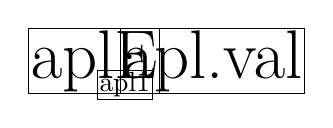
\begin{tikzpicture}
                \node[draw,inner sep=0.8pt] at (0, 0) { \Huge \code{apl}{E} };
                \node[draw,inner sep=0.8pt] at (0.39, -0.3) { \code{apl}{1} };
                \node[draw,inner sep=0.8pt] at (1.505, 0) { \Huge \code{apl}{.val} };
            \end{tikzpicture}
        \end{figure}
       %\pause

        \item O atributo herdado $tp$ (tamanho de ponto) afeta a largura da fórmula e $lg$ é a largura do quadro
       %\pause

        \item A função $\Call{comprimir}{B}$ retorna o tamanho de $B$, reduzido em 30\% e a função $\Call{desloc}{B_1, B_2}$ permite o deslocamento do bloco
            $B_2$ para baixo ao computar a largura do quadro
       %\pause

        \item Esta definição é L-atribuída
    \end{itemize}

\end{frame}

\begin{frame}[fragile]{Esquema de tradução para tamanho e largura de quadros}

\[
    \begin{array}{lcl}
        S\to & & \{ B.tp := 10 \} \\
        & B & \{ S.lg := B.lg \} \\
        B\to & & \{ B_1.tp := B.tp \} \\
        & B_1 & \{ B_2.tp := B.tp \} \\
        & B_2 & \{ B.lg := \max(B_1.lg, B_2.lg) \} \\
        B\to & & \{ B_1.tp := B.tp \} \\
        & B_1 & \\
        & \textbf{sub} & \{ B_2.tp := \Call{comprimir}{B.tp} \} \\
        & B_2 & \{ B.lg := \Call{desloc}{B_1.lg, B_2.lg} \} \\
        B\to \textbf{texto} & & \{ B.lg := \textbf{texto}.l \times B.tp \} \\
    \end{array}
\]

\end{frame}
